\chapter[Metodologia]{Metodologia}
\label{ch:metodologia}

\section{Considerações Iniciais}

Neste capítulo, será apresentada a metodologia utilizada no desenvolvimento dessa 
monografia. Na seção 4.2, será detalhado a metodologia adotada, de acordo com os 
critérios de abordagem, natureza, objetivos e procedimentos. A seção 4.3 acordará o fluxo 
das atividades que foram desenvolvidas nesse primeiro momento do trabalho, e uma projeção das atividades 
que serão desenvolvidas no Trabalho de Conclusão de Curso 2(TCC2). A seção 4.4 abordará a pesquisa bibliográfica.
A seção 4.5 focará na metodologia de desenvolvimento. A seção 4.6 apresenta como será conduzida a análise de resultados. 
Por fim, a seção 4.7 ilustra 
o cronograma das atividades já desenvolvidas ao longo do TCC1, bom como o provável cronograma para 
condução das atividades previstas no TCC2.


\section{Classificação da Pesquisa}

De acordo com \citeonline{gerhardt2009}, a metodologia é o estudo da organização, dos 
caminhos a serem percorridos para se realizar uma pesquisa ou um estudo; ou para se 
fazer ciência. No caso de uma pesquisa científica, ela pode ser classificada em 
vários tipos: quanto à abordagem; quanto à natureza; quanto aos objetivos e quanto aos procedimentos.

\subsection{Quanto à Abordagem}

A classificação quanto à abordagem pode ser dividida em: pesquisa qualitativa e quantitativa. 

A pesquisa qualitativa busca explicar o porquê das coisas e 
comumente analisa dados que não são métricos, tornando difícil 
a quantificação de valores. Ela tende a salientar os
aspectos dinâmicos, holísticos e individuais da experiência humana, para apreender
a totalidade no contexto daqueles que estão vivenciando o fenômeno \cite{gerhardt2009}.

Já a pesquisa quantitativa têm resultados que podem ser quantificados e se baseia na 
análise de dados brutos, tendendo a enfatizar o raciocínio dedutivo, as regras da lógica 
e os atributos mensuráveis da experiência humana

Tendo o conhecimento desses conceitos, nesse trabalho, a pesquisa é, predominantemente, 
qualitativa, por possuir resultados não métricos que precisam de interpretação. 


\subsection{Quanto à Natureza}

Segundo \citeonline{gerhardt2009}, a pesquisa quanto à natureza pode ser dividida em: pesquisa 
básica e pesquisa aplicada. A pesquisa básica gera conhecimentos novos, sem aplicação básica 
prevista, e a pesquisa aplicada gera conhecimentos para aplicação prática, dirigidos à solução de 
problemas específicos. Tendo o objetivo de desenvolver um aplicativo com os conhecimentos 
adquiridos, a pesquisa a ser realizada nesse trabalho é de natureza aplicada.

 
\subsection{Quanto aos Objetivos}

Quanto aos objetivos, \citeonline{gil1991} classifica as pesquisas em exploratória, 
descritivas e explicativas. 

A pesquisa exploratória tem como objetivo o aprimoramento 
de ideias, ou a descoberta de intuições, o que a faz ter um planejamento flexível. 
Essas pesquisas envolvem: (i) levantamento bibliográfico, (ii) entrevistas com pessoas 
que tiveram experiência prática com o problema pesquisado, e (iii) análise de exemplos que 
"estimulam a compreensão".


%A pesquisa descritiva tem como objetivo principal descrever caracteristicas de determinada 
%população ou fenomeno, ou o estabelecimento de relaçoes entre variáveis, definindo técnicas 
%padronizadas de coleta de dados, tais como, questionários e observação sistemática. A 
%pesquisa explicativa têm objetivo principal identificar os fatores que determinam ou contribuem 
%para a ocorrência  dos fenômenos. 

Essa monografia é portanto, predominantemente, exploratória, 
por envolver levantamento bibliográfico e questionários com mulheres que têm experiência 
prática com o problema. A própria definição do tema teve, em si, um caráter intuitivo. 

\subsection{Quanto aos Procedimentos}

\citeonline{gil1991} separa a pesquisa quanto aos 
procedimentos em: experimental; bibliográfica; 
documental; de campo; Ex-Post-Facto; 
de levantamento; com survey; estudo de caso; 
participante; pesquisa-ação; etnográfica e etnometodológica.

Essa pesquisa, quanto aos procedimentos, pode ser classificada como: pesquisa bibliográfica e 
estudo de caso.
Ela é bibliográfica porque utiliza levantamento de referências teóricas já analisadas, 
como livros e artigos científicos. É estudo de caso por 
ser aplicado à comunidade criada pela própria autora, com 
mulheres que tiveram interesse no tema.


\section{Fluxo das Atividades}

O fluxo a seguir foi construído utilizando a notação BPMN, e apresenta 
tanto as atividades já desenvolvidas ao longo da execução do 
TCC1, quanto as que serão desenvolvidas no TCC2. 
Adicionalmente, os próximos tópicos detalharão de 
forma mais específica cada etapa desse processo.

\begin{figure}[ht]
	\centering
	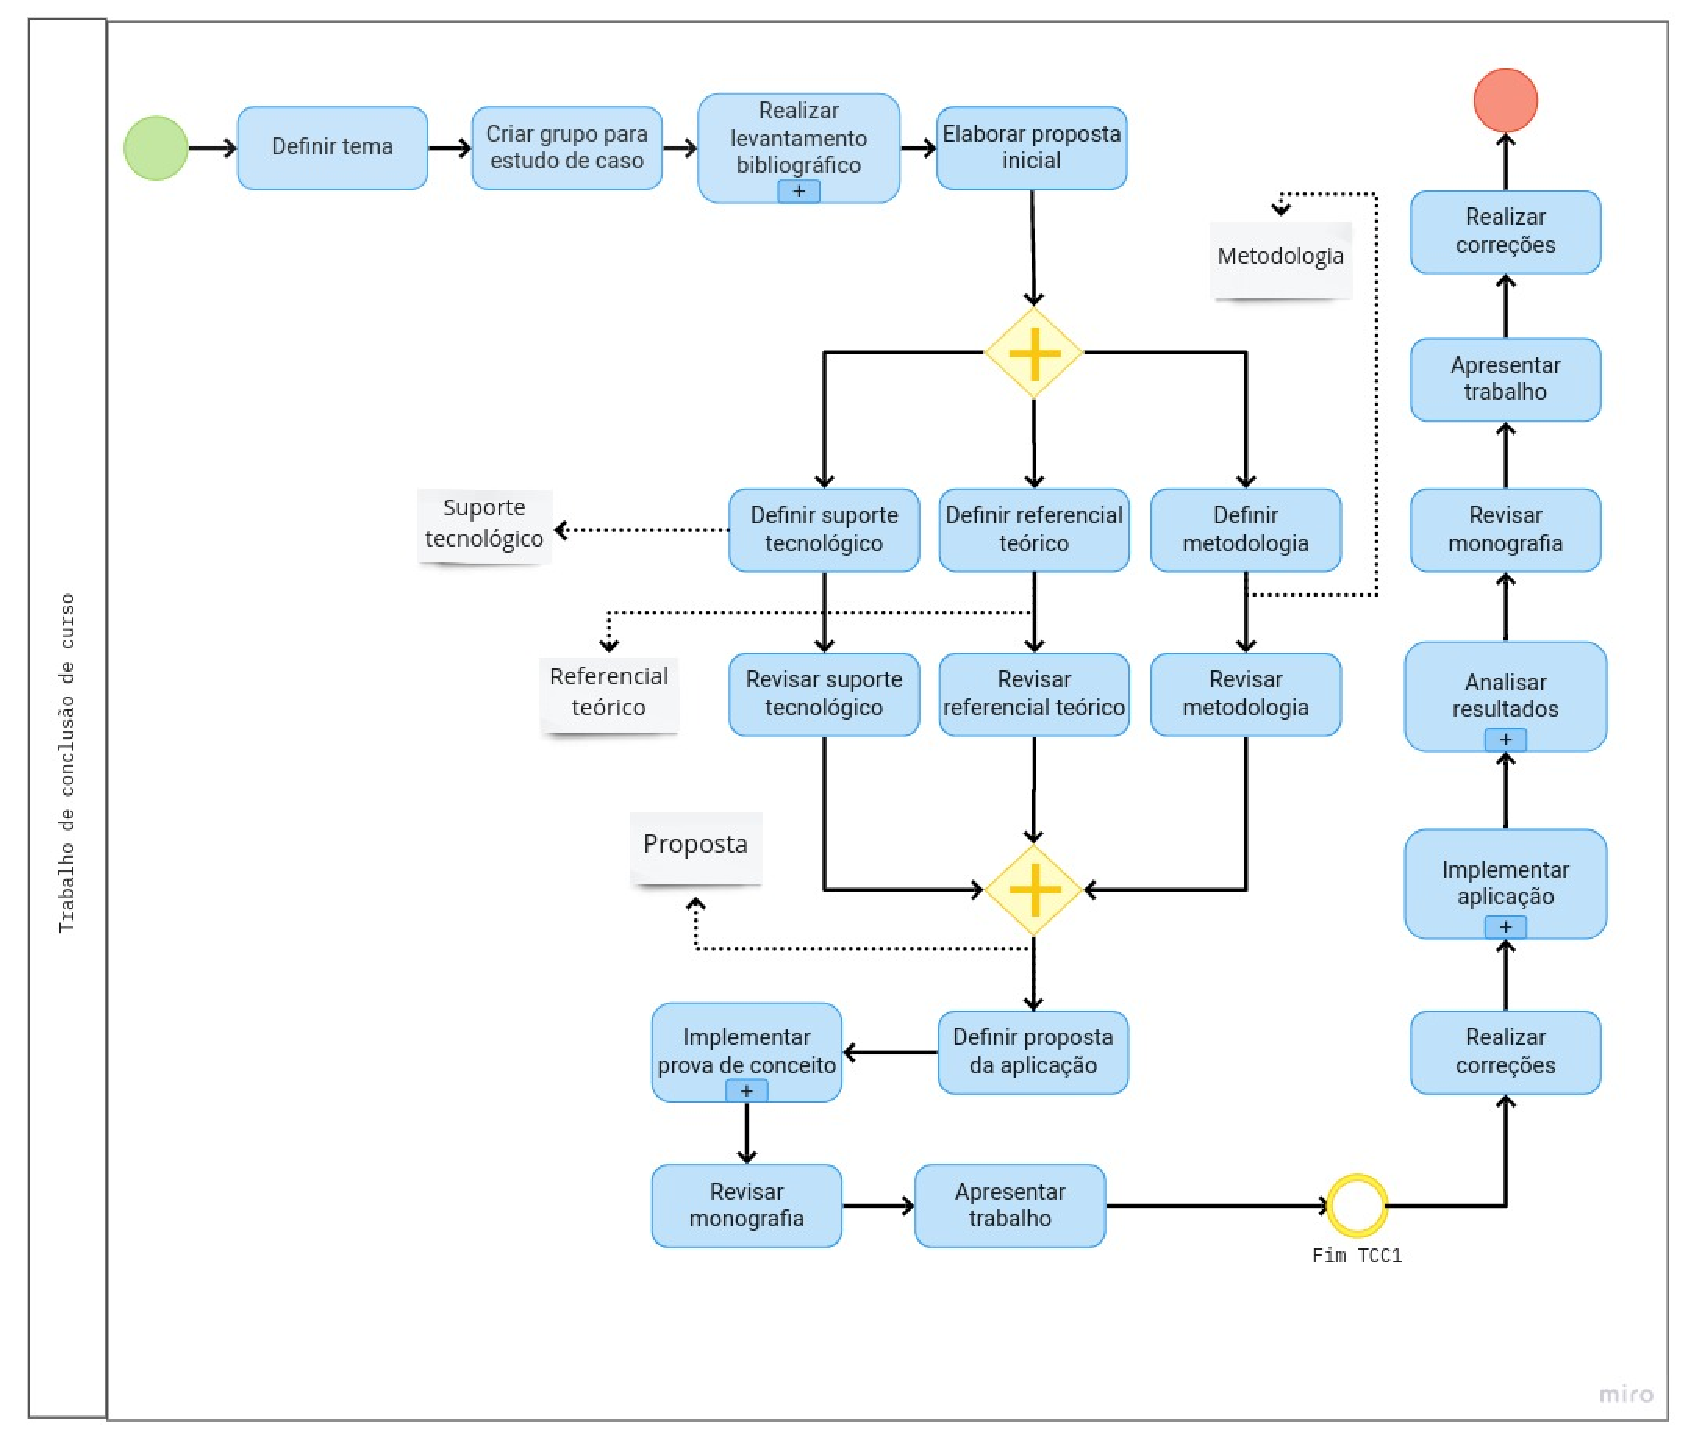
\includegraphics[keepaspectratio=true,scale=0.55]{figuras/fluxodeatividades.pdf}
	\caption{Fluxo das Atividades Desenvolvidas no TCC1 e TCC2}
        \label{fig03}
\end{figure}

\textbf{Definir tema}: o tema foi escolhido, junto aos orientadores, utilizando o ciclo menstrual como domínio e discutindo
possíveis aplicações da engenharia de software sobre o tema. 

\textbf{Criar grupo para estudo de caso}: foi criado um grupo com mulheres em idade fértil e perfis diversos, 
que se interessaram pelo tema e resolveram apoiá-lo. Esse grupo é e será utilizado 
para o estudo de caso.

\textbf{Realizar Levantamento Bibliográfico}: nessa etapa, foi obtido um conhecimento 
inicial do tema e levantadas publicações pertinentes sobre os tópicos dessa monografia. 

\textbf{Elaborar proposta inicial}: nessa etapa, foi elaborada uma proposta inicial que 
atendesse a necessidade da comunidade e conciliasse domínio e engenharia de software. 
Optou-se pela criação de um aplicativo com sistema de recomendação de tarefas baseadas no perfil e
na fase do ciclo menstrual feminino. No capítulo \ref{ch:proposta}, a proposta inicial será mais bem detalhada.

\textbf{Definir suporte tecnológico}: nessa etapa, foram levantadas as tecnologias necessárias para o desenvolvimento da aplicação, 
gerenciamento e pesquisa. Gerou o capítulo \ref{ch:suporte} como artefato.

\textbf{Revisar suporte tecnológico}: o capítulo de suporte tecnológico foi revisado pelos orientadores e foram implementadas as devidas correções e sugestões.

\textbf{Definir referencial teórico}: nessa etapa, foram levantadas as principais fontes conceituais para embasar o presente trabalho. Gerou o capítulo \ref{ch:referencial} como artefato.

\textbf{Revisar referencial teórico}: o capítulo \ref{ch:referencial} foi revisado pelos orientadores e foram implementadas as devidas correções e sugestões.

\textbf{Definir metodologia de pesquisa}: nessa etapa, foi definida a metodologia 
para guiar a pesquisa, permitindo classificar essa última quanto
à abordagem, à natureza, aos objetivos, e aos procedimentos. Gerou como artefato o capítulo \ref{ch:metodologia}.

\textbf{Revisar metodologia de pesquisa}: o capítulo de metodologia foi revisado pelos orientadores e foram implementadas as devidas correções e sugestões.

\textbf{Definir proposta da aplicação}: delimitou-se o escopo da proposta inicial, obtendo um maior detalhamento 
dos objetivos gerais e específicos deste trabalho. Gerou como artefato o capítulo \ref{ch:proposta}.

\textbf{Implementar prova de conceito}: implementou-se parte da proposta, desenvolvendo um protótipo e uma aplicação inicial, com o objetivo 
de avaliar a viabilidade do projeto e das tecnologias escolhidas.

\textbf{Revisar monografia}: toda a monografia foi revisada e as devidas orientações implementadas.
 
\textbf{Apresentar trabalho}: apresentar o trabalho aos membros da banca.

\textbf{Implementar aplicação}: esta atividade será desenvolvida no TCC2 e tem como objetivo 
o desenvolvimento do aplicativo.

\textbf{Analisar resultados}: esta atividade será desenvolvida no TCC2 e tem como objetivo 
analisar os resultados obtidos com a implementação da aplicação, conferindo se ela atende 
aos objetivos gerais e específicos estabelecidos no Capítulo 1 desta monografia.

\section{Pesquisa Bibliográfica}

A pesquisa bibliográfica foi realizada a partir da plataforma do Periódico Capes, utilizando a ferramenta de pesquisa avançada.
Os temas foram separados em duas partes: influências do ciclo menstrual e sistema de recomendação.
Para as influências do ciclo menstrual, vale ressaltar que é um tema ainda pouco abordado na literatura e existem 
várias discrepâncias entre os estudos, por isso foram selecionados aqueles que apoiavam a tese de que 
o ciclo influencia de alguma forma as habilidades cognitivas, motoras e sensoriais. 

%A partir da plataforma Scielo, foi utilizada a seguinte string de busca:

%((((((Menstrual cycle influence) OR (Menstrual cycle)) AND NOT (pregnancy)) AND NOT (sexual) ) AND (phases of the menstrual cycle) AND (phases of the menstrual cycle phases)) AND NOT (teenagers)) AND NOT (sports).

%Ela resultou em 40 artigos e foram feitas leituras parciais dos artigos mais relevantes. A partir desses, três trabalhos foram selecionados para compor a referência bibliográfica desse trabalho.

A partir do periódico capes, foi utilizada a seguinte \emph{string} de busca:
qualquer um que contém \emph{menstrual cycle influence} e qualquer um que contém 
\emph{influence of the phases of the mental cycle}. 

Depois, foi utilizada a ferramenta de filtragem, excluindo artigos que tivessem o tópico, \emph{sex difference} e \emph{male}
 e, adicionando artigos que fossem da coleção Scopus, Science ou Pubmed e periódicos revisados por pares. Dessa busca, surgiram 167 artigos.
Desses, o trabalho mais relevante foi o de \citeonline{poroma2014}. A partir desse estudo, foram selecionados, pela referência bibliográfica, estudos que apoiavam 
a teoria de que o ciclo influenciava em algum aspecto a vida das mulheres, ou explicassem de forma mais teórica o funcionamento do ciclo menstrual.


Para o sistema de recomendação, foi utilizada uma pesquisa mais geral procurando por \emph{recommendation system survey}. Dessa pesquisa, o principal artigo selecionado foi o 
do \citeonline{bobadilla2013}. Por esse artigo, outros estudos foram selecionados utilizando a referência bibliográfica. Com o andamento da escrita, surgiu a necessidade de buscar
por temas mais específicos, tais como: \emph{Hybrid Recommender Systems}, \emph{Collaborative Filtering} e \emph{Content-based filtering}. A tese de mestrado \cite{mauricio} foi adicionada a partir 
de uma conversa com os orientadores, que citaram o trabalho sobre sistema de recomendação realizado por um deles.


\section{Metodologia de Desenvolvimento}

No escopo do TCC1, foi utilizado o Kanban para o gerenciamento das tarefas que foram 
desenvolvidas no decorrer da escrita da monografia, da construção da proposta e do desenvolvimento 
da prova de conceito.

O Kanban é um sistema visual que consiste em um quadro com três colunas: a fazer, em execução e feito (vide Figura \ref{fig04}). 
Dentro das colunas, existem cartões com as tarefas ou ações que precisam ser executadas. As tarefas que devem 
ser desenvolvidas ficam inicialmente na coluna do a fazer. Ao começar o desenvolvimento, elas são alocadas para a coluna 
em execução. Quando finalizadas, as tarefas são movidas para a coluna feito.

\begin{figure}[ht]
	\centering
	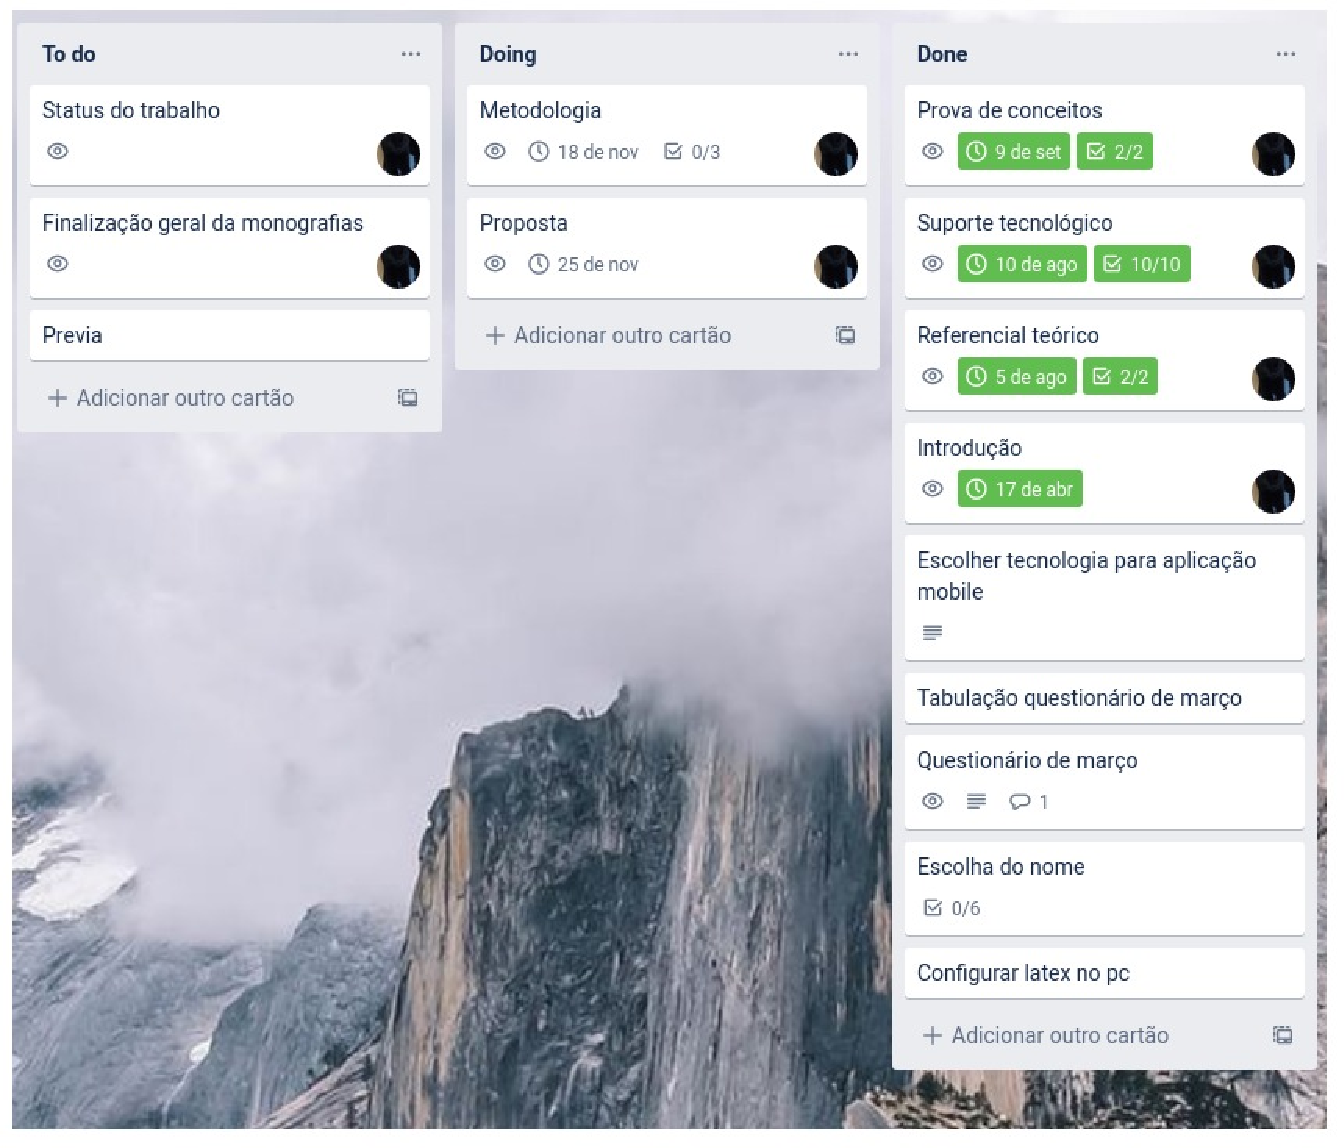
\includegraphics[keepaspectratio=true,scale=0.6]{figuras/kanban.pdf}
	\caption{Kanban das Atividades Desenvolvidas no TCC1 }
        \label{fig04}
\end{figure}

No escopo do TCC2, além do Kanban, que será utilizado para o gerenciamento das tarefas a serem desenvolvidas no TCC2,
também será utilizado um processo baseado em metodologias ágeis, mais especificamente, no Scrum \cite{scrum2017}. O fluxo de desenvolvimento 
pela metodologia Scrum é demonstrado na Figura \ref{fig05}.


\begin{figure}[ht]
	\centering
	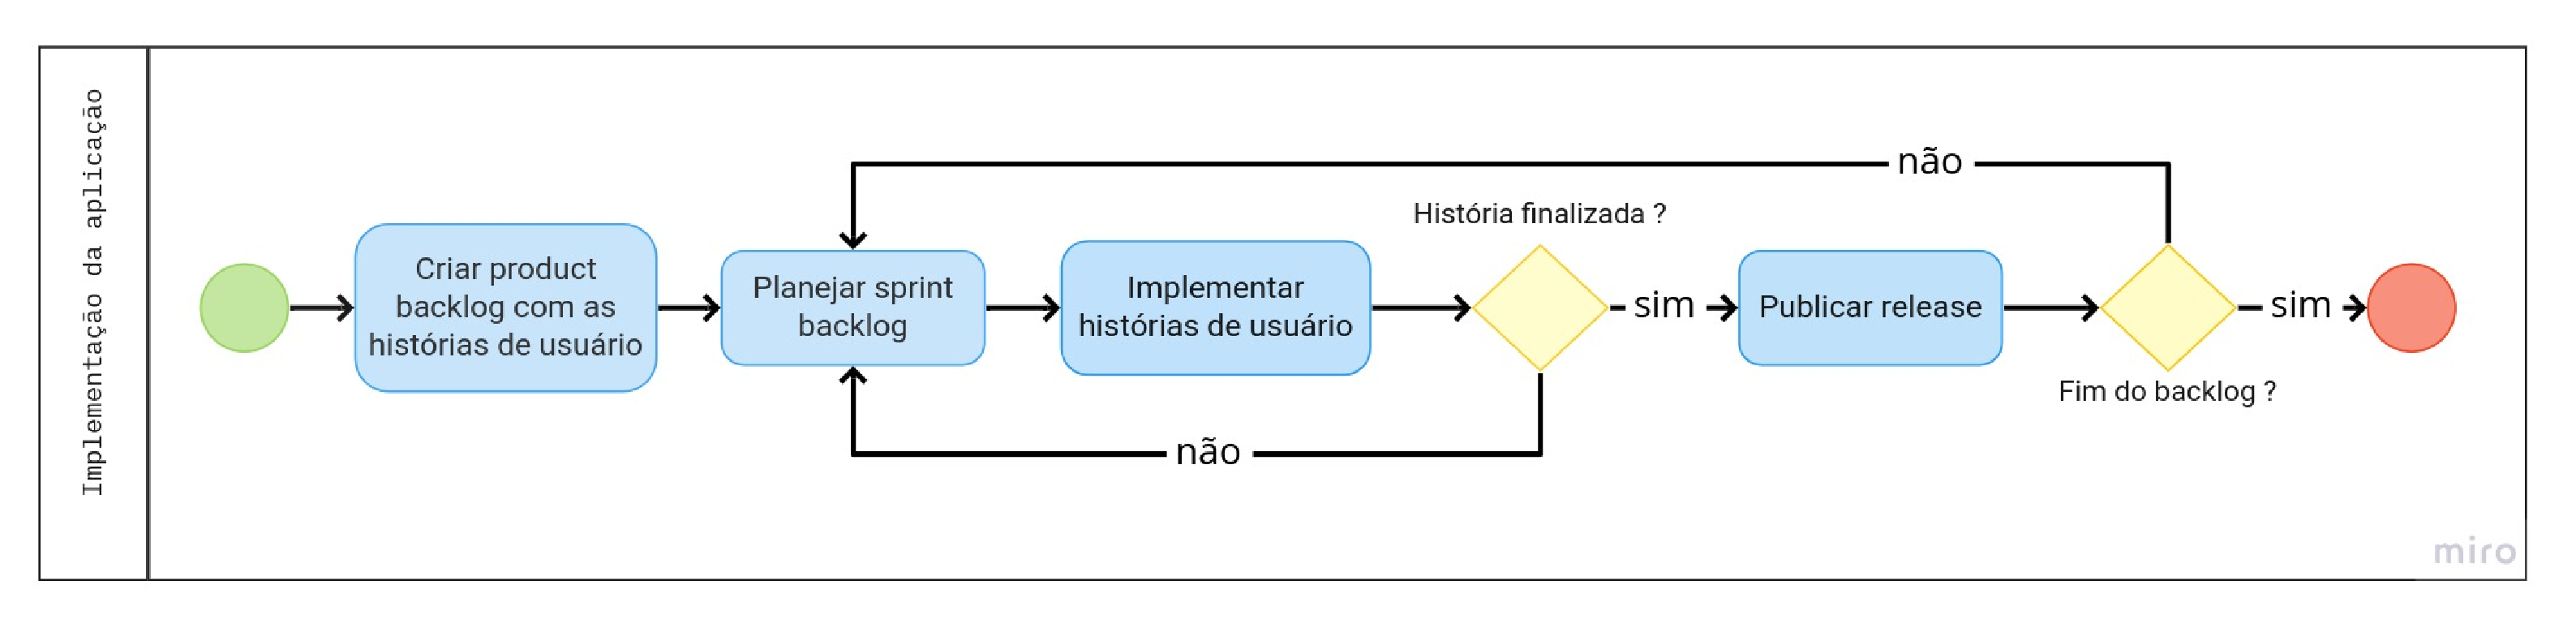
\includegraphics[keepaspectratio=true,scale=0.29]{figuras/scrummet.pdf}
	\caption{Metodologia para o TCC2}
        \label{fig05}
\end{figure}

\textbf{Criar \emph{product backlog} com as histórias de usuário}: criação do backlog separando as histórias de usuário por tema e épico. As histórias de usuário seguirão 
o formato proposto pela metodologia (Eu como ... desejo ... para que eu possa ...). Haverá ainda critérios de aceitação bem definidos. 

\textbf{Planejar \emph{sprint backlog}}: as histórias de usuário do \emph{product backlog} serão mapeadas para serem executadas durante \emph{sprints} de 15 dias.

\textbf{Implementar história de usuário}: as histórias de usuário serão implementadas e só serão finalizadas quando os critérios de aceitação forem cumpridos.

\textbf{Publicar release}: ao final de cada \emph{sprint}, se as histórias de usuário foram executadas, uma nova versão da aplicação será lançada. 

\section{Análise de Resultados}

Segundo \citeonline{gil1991}, o estudo de caso é mais utilizado em estudos exploratórios e descritivos, 
e pode ser importante para fornecer respostas relativas a causas de determinados fenômenos. É definido por sete etapas:
\begin{itemize}
	\item formulação do problema;
	\item definição da unidade-caso;
	\item determinação do número de casos;
	\item elaboração do protocolo;
	\item coleta de dados;
	\item avaliação e análise dos dados; e
	\item preparação do relatório.
\end{itemize}

A formulação do problema foi executada na parte de definição do tema.

A unidade caso é do tipo estudo de caso coletivo. Esse tipo de estudo tem o propósito de estudar características
de uma população, no caso deste trabalho, mulheres em idade fértil.

Para a determinação de números de casos, foram utilizados os múltiplos casos de mulheres em idade fértil que compuseram o grupo de pesquisa criado pela autora. De acordo com o \citeonline{gil1991}, 
o número ideal de casos consiste de quatro a dez casos. O grupo é formado por 22 mulheres inseridas em diferentes contextos.

O protocolo elaborado envolve: visão global do projeto, procedimentos de campo, determinação das questões e guia para a elaboração do relatório.
A visão global do projeto descreve o propósito e o cenário em que será desenvolvido o estudo. Nesse caso, o propósito é a criação de um aplicativo com sistema de recomendação de tarefas baseadas 
em perfil e fase do ciclo menstrual das mulheres. O cenário em que será desenvolvido o estudo é um grupo criado com mulheres que se interessaram pela proposta do trabalho.

O procedimento de campo envolveu acesso à organizações formadas por mulheres, sendo uma delas o pyladies-df. Através dessas organizações, foi possível mobilizar as mulheres 
para a entrada no grupo do estudo de caso.

A determinação das questões foi feita através de conversas com as 
integrantes do grupo bem como com base nos estudos documentados no 
referencial teórico, Capitúlo \ref{ch:referencial}. Isso possibilitou a aplicação de 
um questionário para coleta de dados, descrito no Capítulo 5.

Por fim, a preparação do relatório deu-se após a aplicação do questionário, acordado na etapa anterior
\section{Cronograma}

O cronograma da Tabela \ref{tab04} explicita as atividades executadas com seus respectivos prazos no TCC1, Já a Tabela \ref{tab05} 
explicita as prováveis datas de execução do TCC2.
Para fins de uma visualização mais adequada, foi considerado com a letra \textbf{P}, a
data prevista, e a letra \textbf{E}, para a data Executada.

\begin{table}[ht]
	\centering
	\caption{Atividades do Trabalho de Conclusão de Curso 1}
	\label{tab04}
	
	\begin{tabular}{ccccccc}
		\toprule
		\textbf{Atividades} & \textbf{Março} & 
		\textbf{Julho}  & \textbf{Setembro}& \textbf{Outubro} & \textbf{Novembro} & \textbf{Dezembro}\\
		\midrule
		Definir tema & P-E & & &  &\\
		\midrule
		\begin{minipage} [t] {0.2\textwidth} \centering Realizar Levantamento Bibliográfico \end{minipage} & P-E & E & P & E & & \\
		\midrule
		\begin{minipage} [t] {0.2\textwidth} \centering Elaborar Proposta Inicial\end{minipage} &  & E & P &  &  &\\
		\midrule
		\begin{minipage} [t] {0.2\textwidth} \centering Definir Suporte Tecnológico \end{minipage} & E & P & &  & &\\
		\midrule
		\begin{minipage} [t] {0.2\textwidth} \centering Definir Metodologia de Pesquisa\end{minipage} &  &  & P & E & &\\
		\midrule
		\begin{minipage} [t] {0.2\textwidth} \centering Definir Proposta da Aplicação \end{minipage} &  & & &  & P - E &\\
		\midrule
		\begin{minipage} [t] {0.2\textwidth} \centering Implementar prova de Conceito \end{minipage} &  & E & & E & P-E &\\
		\midrule
		\begin{minipage} [t] {0.2\textwidth} \centering Revisar \end{minipage} &  & & P-E & P-E & P-E &\\
		\midrule
		\begin{minipage} [t] {0.2\textwidth} \centering Apresentar Trabalho \end{minipage} &  &  & &  & & P-E\\
		\bottomrule
	\end{tabular}
\end{table}


O cronograma do TCC1 sofreu muitas alterações devido à pandemia da covid-19. O semestre de 2020/1 estava previsto para iniciar no mês de março e finalizar em julho, mas houve uma pausa no 
mês de março e o retorno ocorreu no mês de agosto. Algumas atividades continuaram sendo desenvolvidas durante essa pausa.



\begin{table}[ht]
	\centering
	\caption{Atividades do Trabalho de Conclusão de Curso 2}
	\label{tab05}
	
	\begin{tabular}{ccccc}
		\toprule
		\textbf{Atividades} & \textbf{Fevereiro} & 
		\textbf{Março}  & \textbf{Abril}& \textbf{Maio}\\
		\midrule
		\begin{minipage} [t] {0.2\textwidth} \centering Realizar Correções da Banca \end{minipage} & P &  &  &  \\
		\midrule
		\begin{minipage} [t] {0.2\textwidth} \centering Implementar Aplicação \end{minipage} & P & P & P &  \\
		\midrule
		\begin{minipage} [t] {0.2\textwidth} \centering Análisar Resultados \end{minipage} &  &  &P &P  \\
		\midrule
		\begin{minipage} [t] {0.2\textwidth} \centering Refinar Monografia \end{minipage} &  &  &  & P \\
		\midrule
		\begin{minipage} [t] {0.2\textwidth} \centering Apresentar Trabalho \end{minipage} &  & & & P \\
		\bottomrule
	\end{tabular}
\end{table}

O cronograma do TCC2 é uma prévia das prováveis datas de entrega das atividades a serem desenvolvidas no semestre de 2020/2.

\section{Considerações Finais do Capítulo}

Este capítulo apresentou como o trabalho foi desenvolvido.

As naturezas desta pesquisa estão sinalizadas pelos quadros amarelos.

\begin{figure}[ht]
	\centering
	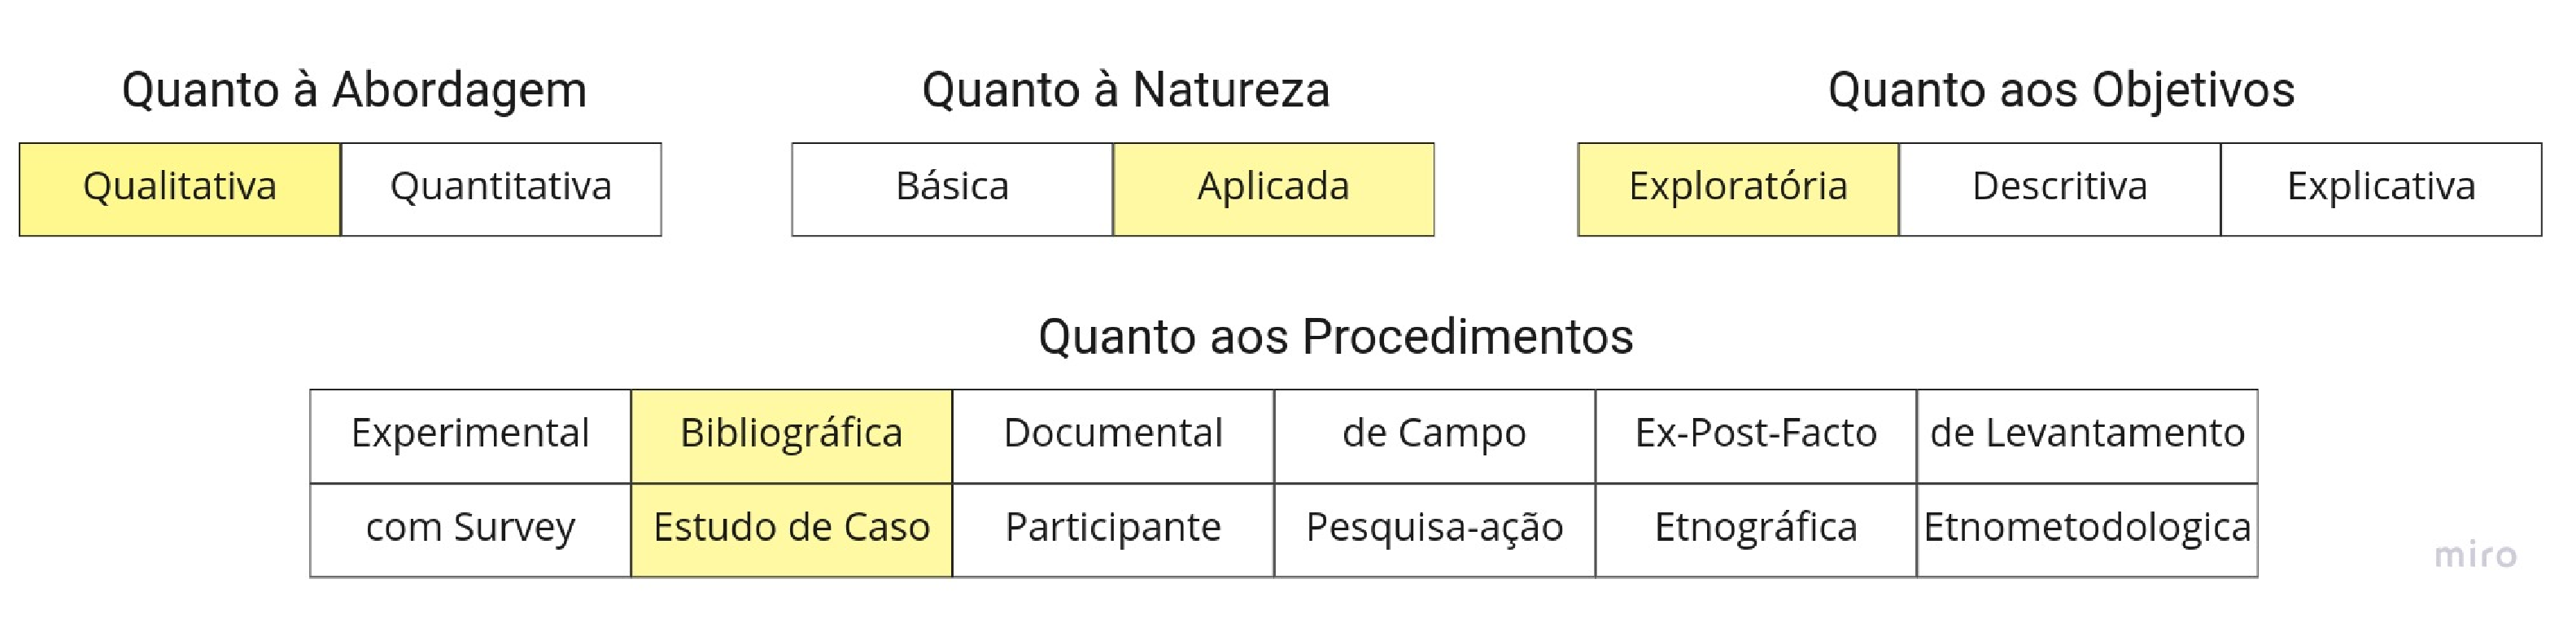
\includegraphics[keepaspectratio=true,scale=0.3]{figuras/resumoAbordagem.pdf}
	\caption{Resumo das Naturezas da Pesquisa}
        \label{fig06}
\end{figure}

Para o gerenciamento das atividades do escopo do TCC1, foi utilizado o Kanban. Como metodologia de desenvolvimento para o TCC2, será utilizada uma adaptação do scrum.

Para a coleta e análise de resultados, foi utilizado um estudo 
de casos aplicado a um grupo de mulheres, sendo esse criado pela 
autora. Cabe ressaltar que a análise de resultados ainda será 
realizada no escopo do TCC2. Portanto, o estudo de casos, com o 
grupo de interessadas, ainda será objeto de estudo.



          
%Do ponto de vista dos procedimentos técnicos esta é uma pesquisa 
%experimental que procura estabelecer uma relação entre as causas e os efeitos de um determinado fenômino. Este fenômeno seria, os efeitos do ciclo menstrual femino na performance individual das mulheres nas tarefas cotididanas.

